\documentclass{as-preprint-template}

\PassOptionsToPackage{hyphens}{url}

\usepackage{fontspec} % Required due to a bug in microtype
\usepackage{amsmath,amsfonts}
\usepackage{booktabs,rotating}
\usepackage{subcaption}
\usepackage{flafter}
\usepackage{tikz}
\usetikzlibrary{positioning}
\usetikzlibrary{decorations.pathreplacing}
\usepackage[inline,shortlabels]{enumitem}

\newcommand{\xvar}[5]{x_{#1, #2, #3}^{#4, #5}}
\newcommand{\yvar}[3]{y_{#1, #2, #3}}
\newcommand{\wvar}[3]{w_{#1, #2, #3}}
\newcommand{\uvar}[2]{u_{#1#2}}
\newcommand{\edit}[1]{#1}
\newcommand{\editt}[1]{#1}

\graphicspath{{./figures/}}

\usepackage[backend=biber,style=authoryear,dashed=false,maxbibnames=99,citestyle=authoryear,hyperref=true]{biblatex}
\addbibresource{vf.bib}

\usepackage[nameinlink,noabbrev]{cleveref}

\addAuthor{Alberto}{Santini}{Universitat Pompeu Fabra, Barcelona, Spain\thanks{alberto.santini@upf.edu}}
\addAuthor{Enrico}{Bartolini}{RWTH Aachen University\thanks{bartolini@dpo.rwth-aachen.de}}
\addAuthor{Michael}{Schneider}{RWTH Aachen University\thanks{schneider@dpo.rwth-aachen.de}}
\addAuthor{Vinicius}{Greco de Lemos}{University of Twente\thanks{v.grecodelemos@student.utwente.nl}}
\setTitle{The Crop Growth Planning Problem in Vertical Farming}
\setJournal{European Journal of Operational Research}
\setYear{2021}
\setDoi{10.1016/j.ejor.2021.01.034}
\setUrl{https://www.sciencedirect.com/science/article/abs/pii/S0377221721000643}

\begin{document}

\printCover{}
\newpage{}
\maketitle

\begin{abstract}
    In this paper, we study the problem of planning the growth of crops on shelves in vertical farming cabinets under controlled growth conditions.
    By adjusting temperature, humidity, light, and other environmental conditions in different parts of the cabinets, a planner must ensure that crop growth is able to satisfy some deterministic demand.
    We prove this problem to be \(\mathcal{NP}\)-hard and propose an integer programming formulation able to capture real-life operational characteristics, including changes of growth conditions on a daily, shelf-by-shelf basis, over a planning horizon of months.
    We compare four objective functions from which a planner can choose, depending on the specific operations of the company.
    A computational study on realistic instances, which we make available as a public dataset, shows that the choice of objective function heavily influences both the difficulty of solving the model with a standard solver and the solution characteristics.
\end{abstract}

\section{Introduction}

The stocks of arable land per person are declining worldwide, due to increasing population and urbanisation rates, decreasing water availability, and climate change~\autocite{fedoroff2015food}.
Increasing land use for standard agricultural practices has undesirable effects, such as deforestation, an elevated use of fertilisers and pesticides, soil degradation and its eventual depletion, low yield per unit of surface, and extensive transportation costs to move produce from the production to the consumption site~\autocite{benke2017future}.
All these effects take their toll both economically and, more importantly, on the environment and the well-being of urban and rural communities alike.
The large-scale increase in food demand forecast to take place within the next decades has prompted the investigation of alternative production methods.
The main aim of these efforts is to increase the yield per square meter while reducing negative effects on the environment and being economically viable~\autocite{beacham2019vertical}.

\begin{figure}\centering%
    \includegraphics[width=.75\textwidth]{hydroponics.jpg}
    \caption{Stacks of shelves in which mulberries are growing in a hydroponic system, i.e., receiving their nutrients directly from water, without soil. Photograph by Satoshi Kinokuni, distributed under a CC-BY-2.0 license.}\label{fig:hydroponics}
\end{figure}

One of the new production methods which is gaining considerable traction is \emph{Vertical Farming} (VF), i.e., growing crops in vertical stacked layers rather than on the ground~\autocite{beacham2019vertical}.
\Cref{fig:hydroponics} shows three stacked layers hosting mulberry plants.
Each shelf provides the plants with nutrients; in the case depicted in the figure, the plants grow without soil and absorb the nutrients directly from water (a growth method known as hydroponics).
The shelves also provide light, ventilation and, optionally, controlled temperature and CO\textsubscript{2} levels.
The size of the stacks can vary considerably and spans from small shelf cabinets to entire plant factories~\autocite{kozai2018smart,kozai2015plant}.
Their hosting structures range from specially-built buildings to shipping containers and from reused pre-existing buildings to cabinets no larger than a standard refrigerator.

A desirable property of the host structure is that it is isolated from the external environment.
This allows the plants to grow in a \emph{controlled environment} (CE) with regulated levels of light, water, and humidity that can even vary on a shelf-by-shelf basis.
One of the advantages of CE systems is that they are independent of external weather and light conditions and can thus be used in a variety of regions: they are not affected by floods, droughts, and other catastrophic events.
They also allow for minimal interaction with the outside environment, sheltering the crops from parasites, pathogens, or heavy metals (all common occurrences in open-air farming) and thus eliminating the need for pesticides and herbicides.
Final commercial users, such as restaurants, food markets, or hotels, can accommodate the cabinets on their premises, reducing or eliminating any transport cost and the resulting negative effects on the environment.
Crops growing in CE are also not affected by seasonality, and the operators can plan their production to match the demand all year round~\autocite{benke2017future}.
    
On the negative side, growth in a CE is more expensive in terms of energy than open-air farming due to the need of constant artificial lightning.
In recent years, however, the energy footprint of CE systems has improved thanks to low-consumption LED lights and the increased efficiency of on-site renewable energy production and storage.

VF offers opportunities that contribute to achieve the Sustainable Development Goals of the United Nations~\autocite{SDGs}: \emph{Goal 2: Zero Hunger} can be supported by large-scale VF systems producing staple foods in large quantities in countries with restricted space availability or hostile conditions for open-air farming, while the ability of VF systems to reduce the negative effects of traditional farming as described above can play a role in achieving \emph{Goal 12: Responsible Consumption and Production} and \emph{Goal 15: Life On Land}.
Moreover, we note that in pandemic situations like the outbreak of COVID-19, VF systems may offer the additional autonomy and independence from transport operations that is necessary to implement quarantine measures in affected areas.

\subsection{Problem description}

\edit{
    We consider the problem of a planner who must operate a VF cabinet to grow crops and meet some deterministic future demand.
    Each cabinet is composed of a set of stacked shelves, which can host the crops during their growth cycle.
    Industry-grade cabinets allow to specify the growth conditions of each shelf individually, and may vary it day by day.
    The planner must define the growth conditions (temperature, light, humidity) of each shelf, for every day of the planning horizon, keeping in mind that changing configurations too frequently can lead to mistakes and reduce the energy efficiency of the system (for example, swapping back-and-forth between colder and hotter temperatures).
}

\edit{
    The planner must also decide in which shelf they will place each plant, making sure that the receiving shelf has the right conditions for the current growth phase of the plant.
    Growth times of crops under controlled conditions are predictable, and therefore, the planner will plant with suitable advance depending on the days in which there is demand for each crop.
    In other words, the planner does not have to choose the growth start time or the sequence of crops to grow because both are predetermined by the demand.
    Another factor influencing the allocation of crops to shelves is that shelves have limited capacity, which can vary depending on the growth medium used (e.g., hydroponics, aeroponics, peat, synthetic material).
}

\edit{
    The planner can also move plants from one shelf to another during their growth, however, too many movements can damage the crops.
    For example, moving plants can be beneficial to consolidate in the same shelf plants requiring the same growth conditions, but that are currently located in different shelves;
    in this way, the planner can empty shelves to use for growing other crops requiring different conditions.
}

\edit{
    In the days with demand, the planner will harvest the required plants.
    In case demand is too high compared to the size of the cabinet, the planner can decide to reject some orders and not meet part of the demand.
    An easy way to ensure demand is met is to build larger cabinets, but this would lead to higher building and operating costs.
    Thus, the planner might also want to know what is the optimal size of their cabinet, given some future demand.
}

\edit{
    To meet the diverse requirements outlined above, we propose and study four possible goals that a planner can find useful:
    \begin{enumerate*}[(i)]
        \item maximise the demand met, given a fixed number of cabinets;
        \item minimise the number of times shelf configurations change;
        \item minimise the number of times crops move between shelves;
        \item minimise the number of shelves required to meet a given demand.
    \end{enumerate*}
}

\edit{We call this problem the Crop Growth Planning Problem (CGPP).}

\subsection{Contribution}

The main contributions of this paper are the following.
\begin{itemize}
    \item To the best of our knowledge, we are the first to consider the problem of optimally planning the growth of crops in VF cabinets.
    The relevance of this problem stems from the social, environmental, and economic challenges to which VF offers a viable solution, as outlined above.
    \item We incorporate real-life constraints determined by crop growth conditions and the available infrastructure.
    Our model is flexible enough to allow for the growth conditions to change daily and on a shelf-by-shelf basis.
    Growers require such a degree of flexibility to provide the crops with ideal growth conditions and maximise the quality of their yield.
    \item We formalise the CGPP and provide a complete Integer Linear Programme (ILP), proposing four models that differ in their objective functions as outlined above, and decision makers can choose the objective function most suitable for their needs. \edit{We prove that the problem is \(\mathcal{NP}\)-hard, independent of the objective function used.}
    \item We perform an extensive computational study to compare the performance of the models, to determine the size of problem instances solvable via standard solvers, and to compare the operational effects of choosing different objective functions.
    We use a realistic dataset with instances containing up to six crops, twelve shelves, and a time horizon of 100 days.
    We conclude that the objective function has a large effect on the difficulty of solving the problem.
    Moreover, solutions obtained optimising with regards to one objective typically fare poorly with respect to the other objectives.
\end{itemize}

After providing an overview of the literature in \Cref{sec:literature}, we formalise the CGPP and frame it as an ILP in \Cref{sec:models}.
In \Cref{sec:results}, we present the outcome of extensive experiments on realistic instances, providing computational results and managerial insights.
We conclude and point out future research directions in \Cref{sec:conclusions}.

\section{Literature review}\label{sec:literature}

The literature on the topic of crop production planning in VF is scarce.
The only work we are aware of is that of~\textcite{potts2017vf}, who use Operational Research techniques for scheduling crops in shelf cabinets.
The work stems from an industry collaboration with a local business and has not been published as a technical report or journal paper.
The authors study the problem of minimising unmet demand in a growing cabinet in which each shelf can be subject to different lightning and irrigation conditions.
Another decision is the growing medium to assign to each shelf, which influences both its capacity and which crops can grow on the shelf.
The main difference with the CGPP lies in the presence of a scheduling component in the work of ~\textcite{potts2017vf} because the crop growth length can vary within a given time window.
The authors use an ILP to precisely describe the problem.
The ILP is large (for example, it uses four set of variables, three of which are five-indexed), and although the model is not explicitly provided in their presentation, the authors report that it can solve instances with 3 crops and a 70-day planning horizon, but it is not able to solve a problem with 5 crops within 1 day of computing time.
To tackle realistically-sized instances of the problem, the authors use a heuristic that decomposes the problem into two subproblems.
The first tries to minimise unmet demand while satisfying capacity constraints, but it does not allocate crops to shelves.
The second subproblem performs the actual allocation, minimising the number of movements. Thus, the problem has a hierarchical objective function.
Because the second subproblem is still computationally challenging, the authors solve it with a rolling-horizon heuristic.
Using this approach, they are able to obtain solutions of instances with up to 9 crops, 15 shelves, and a planning horizon of 70 days.

\edit{
    As already noted by~\textcite{potts2017vf}, the problem of planning the growth of crops in VF has superficial similarities with machine scheduling problems.
    In particular, we can consider each shelf as a machine, and each crop growth phase as a task required to complete a job.
    Under this analogy, the CGPP has similarities with parallel machine scheduling~\autocite{pms_survey2,pms_survey1} (because shelves work in parallel), parallel machine scheduling with splitting jobs~\autocite{pms_sj} (because units of the same crop can grow on different shelves), scheduling with batching~\autocite{potts2000scheduling} (because different crops can share the same shelf when requiring a common configuration), and job shop scheduling~\autocite{jss,jain1998state} (because each crop must go through its growth phases in a given order).
    Under scheduling terminology, crop growth is non-preemptive because it cannot stop and resume at a later time, and machines are capacitated because each shelf can host a maximum amount of crop units.
}%
\editt{
    From this viewpoint, the CGPP has particular similarities with hybrid flow shop scheduling problems (see, e.g, \textcite{Ruiz_2010} for a comprehensive survey) because each crop may be viewed as a job that must be processed non-preemptively through a predefined sequence of stages (its growth phases), and multiple machines (the shelves) are available at each stage.
}

\edit{
    However, the CGPP also exhibits considerable differences with respect to classical scheduling problems, and cannot be modelled as such.
    The main difference is that scheduling problems involve two sets of decision: first, assigning tasks to machines; second, sequencing and timing tasks on their assigned machines.
    In the CGPP, the second part is missing because the sequence of growth cycles is fixed, and the demands and the lengths of growth determine in advance the planting and harvesting times. 
}%
\editt{
    Returning to the analogy with hybrid flow shops, this means that no scheduling decision, in the classical sense, is required at any stage.
    In fact, for each job (crop) and each point in time it is known a priori whether the job will be processed at that time.
    Rather, because crops can be moved from one shelf to another without interrupting their growth, the decisions to be taken at each stage are whether or not each machine (shelf) is used and to which machine each job is assigned.
    This is a simplifying factor compared to scheduling problems.
    On the other hand, a specific difficulty of the CGPP (besides the fact that shelves are capacitated) is that shelves must be configured at each stage to be compatible with the crops that they host.
    As the analysis in Section~\ref{ssec:complexity} suggests, this aspect seems to be the main complexity driver in CGPP.} 

\edit{
    Another fundamental difference \editt{with respect to classical scheduling problems} lies in the objective functions considered.
    Typical objectives of scheduling problems involve penalties related to makespan, tardiness or earliness; i.e., it is the time at which jobs end which influences the objective cost. In the CGPP these objectives do not apply because crop demand determines the finishing times of jobs.}

\edit{
    Other characteristics which separate the CGPP from classical problems are the following:
    \begin{itemize}
        \item Our machines (the shelves) can be reconfigured and, thus, perform a wide variety of tasks.
        Although some flexible manufacturing systems allow a certain level of machine adaptability (see, e.g., \autocite{logendran1997tabu}), in most production environments, each machine has a specific function and a limited set of tasks it can perform.
        \item The CGPP is different from machine scheduling problems with preemption because crop growth cannot be put on hold.
        Although crops can be moved to any shelf as often as desired, the moves are immediate and there is no break in between.
        On the other hand, when preemption is allowed in scheduling problems, tasks are normally required to resume on the same machine where they stopped (see, e.g., \autocite{LIU2002107,pre1}) after a setup time.
        In the CGPP, setup times (i.e., the time needed to plant crops in a shelf) are generally negligible because our unit of time discretisation is a day.
        \item Machines are capacitated, but their capacity is not fixed and rather depends on the configuration used at a given moment.
        By contrast, in most capacitated job shop, flow shop or lot sizing models, machine capacities are either fixed or can increase by paying a (overtime) penalty (see, e.g., \autocite{buschkuhl2010dynamic,ramezanian2013mathematical}). 
        \item Although each job is made up of a sequence of tasks (the growth phases), in principle a single machine could carry out the whole job if reconfigured to follow the requirements of the crop during its different phases.
        In typical job shop and flow shop problems, including their flexible variants, different tasks require different machines.
    \end{itemize}
}

\editt{In terms of its combinatorial structure, the CGPP has closer ties to multicommodity fixed-charge network flow models, which becomes evident in the formulations presented in Section \ref{sec:models}. Solutions of these models can indeed be interpreted as multi-commodity flows through a time-expanded network in which the nodes are associated with indicator variables and capacity constraints.  There is a vast amount of applications that have been modelled and addressed as multicommodity (fixed-charge) network flow problems (see e.g., \autocite{Magnanti_1984, Ahuja_1993, Batta_2013}), and a detailed review is beyond the scope of this paper. However, we are not aware of applications similar to the one addressed in this paper.}
\edit{
    \editt{For example,} our scenario also differs from lot sizing problems~\autocite{BRAHIMI2017838,lsr} \editt{(or similar problems which include a lot-sizing component and can be modeled as fixed-charge network flow problems)} because we have no inventories and no setup, inventory or backlogging costs.
    Seeds and seedlings are inexpensive to store, so we need not consider raw material inventories; produce is perishable, so there cannot be any finished product inventory; growth is uninterruptible, so there is no intermediate product inventory.
    Also, because of the efficiency of VF and the use of high-yield crops with a high value per unit of weight, the marginal cost for unmet demand is high and deliberate stockout is never an economic option.
    This means that production costs are sunk, and we should aim at producing as much as possible; only when demand is higher than capacity, we can perform a selection of which crops to grow, trying to stock-out on the least profitable crops (see \Cref{ssec:unmet}).
}

We conclude that no other planning problem investigated in the literature adequately captures the specificity of growing crops in VF cabinets.
Hence, the necessity exists to develop new, dedicated mathematical formulations for this problem.
  
\section{Mathematical models}\label{sec:models}

\edit{To formalise the CGPP, we introduce the following notation.}
We consider a set \(C\) of crops that grow on a set \(S\) of shelves during a time horizon \(D = \{1, \ldots, \bar{d}-1\}\).
Each element of \(D\) represents one day; \(\bar{d}\) is the last day when harvest is possible, and \(\bar{d}-1\) is the last day when growth is possible (assume that crops are harvested at the beginning of the day).
We also consider the extended time horizon \(D' = \{0\} \cup D\), where we use day 0 to model seeds not yet planted, which will start growth on day 1.
On each day \(d \in D \cup \{\bar{d}\}\), we have to meet a demand of \(p_{cd}\) units for each crop \(c \in C\) (with \(p_{cd} \in \mathbb{N}\)).

A parameter \(\delta_{cs} \in \{0,1\}\) determines compatibility between crops and shelves, taking value 1 iff crop \(c \in C\) is able to grow on shelf \(s \in S\).
For example, some shelves could be not deep or tall enough for growing certain crops.
In addition, we define the set of shelves compatible with each crop as \(S_c = \{s \in S \ : \ \delta_{cs} = 1\}\).

Furthermore, a crop goes through different phases in its growth, each requiring precise conditions, such as temperature level, humidity, and growth medium characteristics.
One unit of crop \(c\) grows for \(\gamma_c\) days, i.e., it has to spend \(\gamma_c\) days in the VF system.
On each day of growth \(g \in \{1, \ldots, \gamma_c\}\), we require the system to keep the shelf that hosts the unit at condition \(k_{c,g} \in K\), where \(K\) is the set of possible conditions for the shelves.
Practically, \(K\) is the set of all feasible combinations of parameters for soil type, temperature, humidity, CO\textsubscript{2}, air flow, etc.
In real-life applications, the required conditions do not change on a daily basis but only when the crop changes from one \emph{growth phase} to the next, such as germination, seedling growth, etc.
The conditions also affect the shelf capacity, i.e., the number of units of crops that can grow on the shelf simultaneously.
We denote the capacity of a shelf \(s \in S\) under conditions \(k \in K\) as \(q_{sk}\), with \(q_{sk} \in \mathbb{N}\).
Note that the capacity refers to the total number of units of \emph{any} crop that can grow on the shelf at the same time, thereby allowing mixing different crops on the same shelf.

\edit{In practice, growers tend to avoid moving plants too much and, both for simplicity and to reduce movements, try to place plants on shelves which will be able to accommodate them for their entire growth cycle.
However, it is easy to model a situation in which plants can start growth on a short shelf but later need a taller shelf by making the compatibility parameter \(\delta_{cs}\) introduced above dependent on the growth day \(g\).}

For modelling convenience, we extend the set \(S\) with two dummy shelves, obtaining set \(S' = \{ \sigma, \tau \} \cup S\) and sets \(S'_c = \{\sigma,\tau\} \cup S_c\).
Element \(\sigma\) represents the \emph{seed vault}, i.e., a virtual location for units of crop before they enter the VF system.
Analogously, \(\tau\) represents the \emph{produce storage}, i.e., the virtual location where units of crop go when they are ready for pick-up.
Furthermore, we denote as growth day \(0\) the last day a unit of crop is in the seed vault.
In other words, the set of extended growth days for a crop \(c\) is \(\{0, 1, \ldots, \gamma_c \}\).

Because commercial VF cabinet shelves are often not all different, we can reduce the size of the model by considering the set \(T\) of shelf types.
Shelves of the same type have the same compatibility with crops and the same capacities.
We can then use parameters \(\delta_{ct} \in \{0,1\}\) for compatibility between crop \(c \in C\) and shelves of type \(t \in T\), and \(q_{tk} \in \mathbb{N}\) to denote the capacity of any shelf of type \(t\) under condition \(k \in K\).
Analogously, we can define sets \(T' = \{\sigma,\tau\} \cup T\), \(T_c = \{t \in T \ : \ \delta_{ct} = 1\}\), and \(T'_c = \{\sigma,\tau\} \cup T_c\).
We denote as \(n_t\), with \(n_t \in \mathbb{N}\), the number of shelves of type \(t \in T\) available in the VF system.

We use two sets of variables:
\begin{itemize}
    \item \(\xvar{t_1}{d}{t_2}{c}{g} \in \mathbb{N}\) is the number of units of crop \(c \in C\) in their \(g\)-th day of growth (\(g \in \{0, \ldots, \gamma_c\}\)), growing on shelves of type \(t_1 \in T'_c\) on day \(d \in D'\) and going to shelves of type \(t_2 \in T'_c\) on day \(d+1\).
    \item \(\yvar{t}{d}{k} \in \mathbb{N}\) is the number of shelves of type \(t \in T\) with configuration \(k \in K\) on day \(d \in D\).
\end{itemize}

\begin{figure}
    \centering
    
    \resizebox{0.75\textwidth}{!}{%
\tikzset{>=latex}
\begin{tikzpicture}
    \foreach \x in {0,...,7}
        \node at (2 * \x, 10) {\(d=\x\)};

    \node at (-2, 8) {\(\sigma\)};

    \foreach \y in {1,...,3} {
        \pgfmathtruncatemacro{\ylabel}{4-\y}
        \node at (-2, 2 * \y) {type \ylabel};
    };

    \node at (-2, 0) {\(\tau\)};

    \foreach \x in {0,...,7}
        \foreach \y in {0,...,4}
            \draw[black,fill=black] (2 * \x, 2 * \y) circle (.5ex) node (p\x\y) {};

    \path[->,dashed]
        (p04) edge (p13)
        (p13) edge (p23)
        (p23) edge (p33)
        (p33) edge (p41)
        (p41) edge (p51)
        (p51) edge (p60);

    \path[->,dotted]
        (p24) edge (p33)
        (p33) edge (p43)
        (p43) edge (p52)
        (p52) edge (p62)
        (p62) edge (p70);

    \node[below left=-.1cm and -.3cm of p13] {\small \(k_1\)};
    \node[below left=-.1cm and -.3cm of p23] {\small \(k_1\)};
    \node[below left=-.1cm and -.3cm of p33] {\small \(k_1\)};
    \node[below left=-.1cm and -.3cm of p43] {\small \(k_1\)};
    \node[below left=-.1cm and -.3cm of p41] {\small \(k_2\)};
    \node[below left=-.1cm and -.3cm of p51] {\small \(k_2\)};
    \node[below left=-.1cm and -.3cm of p52] {\small \(k_3\)};
    \node[below left=-.1cm and -.3cm of p62] {\small \(k_3\)};
\end{tikzpicture}}

    \caption{
        Time-expanded graph whose columns represent days, and rows represent shelf types.
        The two arrow paths (dashed and dotted) show two crops growing in the system.
        The labels next to the nodes represent the shelf configurations.
    }\label{fig:time-expanded}
\end{figure}

It is helpful to visualise the shelves (as shelf types) and the time horizon as a time-expanded graph, in which paths represent movement of crops while growing.
\Cref{fig:time-expanded} depicts an example with three shelf types, two crops (represented by the dashed and dotted paths, respectively), and no compatibility constraints.
The first crop needs to spend three days on a shelf with configuration \(k_1\), followed by two days on a shelf with configuration \(k_2\).
If we have demand for this crop on day 6, this means the growth needs to start at the beginning of the time horizon and, in fact, the crop leaves the seed vault on day 0 and is already growing on a shelf of type 1 on day 1.
The second crop needs four days in the system: during the first two, it needs a shelf with configuration \(k_1\), and during the second two, a shelf with configuration \(k_3\).
In this example, we assume that the total number of units we are growing does not exceed the capacity of the shelves of type 1 (in configuration \(k_1\)), and both crops can be present at the same time on these shelves on day 3.

In the following, we describe in detail a mathematical base model that uses an aggregation of shelves into shelf types.
For certain objective functions we must modify the model to introduce new variables or index existing ones on the shelves instead of the shelf types; in this case, we will explain how to set up alternative models.
We present the constraints of the model in \Cref{ssec:constraints} and discuss the possible objective functions in \Cref{ssec:objf}; the reader can also find complete models in the appendix.
\Cref{ssec:varfix,ssec:validineq} explain how to strengthen the base model by fixing variables and adding valid inequalities, respectively.
Finally, in \Cref{ssec:complexity} we prove that the CGPP is \(\mathcal{NP}\)-hard.

\subsection{Constraints}\label{ssec:constraints}

In the following, we describe the constraints to ensure that we satisfy demand and respect capacity limits and shelf condition compatibility.
\begin{description}
    \item[Demand satisfaction] implies that the correct amount of units of crop reach the produce storage on time:
    \begin{equation}
        \sum_{t \in T_c} \xvar{t}{d-1}{\tau}{c}{\gamma_c} = p_{cd} \quad
        \forall c \in C, \forall d \in D \cup \{\bar{d}\}\textrm{.} \label{eq:demand}
    \end{equation}
    \Cref{eq:demand} guarantees that an amount of units of crop \(c\) equal to the demand on day \(d\) is sent from any shelf (where it was on day \(d-1\)) to the produce storage.
    \item[Capacity constraints] ensure that a feasible amount of units of crops is grown on any given shelf, on any given day. Recall that shelf capacities are not fixed but depend on the specific configuration used.
    We can calculate the number of units of crops on shelves of type \(t_1\) with configuration \(k\) on a given day \(d\) by counting, for example, how many units move out from these shelves, i.e., summing over outgoing arcs.
    \begin{equation}
        \sum_{t_2 \in T'} \sum_{\substack{c \in C \\ \delta_{c t_1} = 1 \\ \delta_{c t_2} = 1}} \sum_{\substack{g \in \{1,\ldots,\gamma_c\} \\ k = k_{c,g}}} \xvar{t_1}{d}{t_2}{c}{g} \leq
        q_{t_1 k} \cdot \yvar{t_1}{d}{k} \quad
        \forall t_1 \in T, \forall d \in D, \forall k \in K\textrm{.} \label{eq:capacity}
    \end{equation}
    Note how \cref{eq:capacity} also serves as a linking constraint, forcing variables \(y\) to take non-zero value for a type-day-configuration combination when there are \(x\) variables using a shelf of the given type, with the given configuration, on the given day.
    \item[Planting constraints:] Because the demand determines when the operator needs to harvest a crop, and crop growth lasts a fixed number of days, demand indirectly also determines when the operator will plant the crops.
    \begin{equation}
        \sum_{t \in T_c} \xvar{\sigma}{d - \gamma_c - 1}{t}{c}{0} = p_{cd} \quad
        \forall c \in C, \forall d \in \{ \gamma_c + 1, \ldots, \bar{d} \}\textrm{.}
        \label{eq:planting}
    \end{equation}
    \item[Flow-balance constraints:] While \cref{eq:demand} constrains arcs inbound to the produce storage and \cref{eq:planting} constrains arcs outbound from the seed vault, the following set of constraints refer to arcs to and from non-dummy shelves.
\edit{They ensure that any amount of crop growing on shelves of one type on a given day is sent to the same shelf or other shelves for the next day.}
 \begin{equation}
        \sum_{t_2 \in T'_c} \xvar{t_2}{d-1}{t_1}{c}{g} =
        \sum_{t_2 \in T'_c} \xvar{t_1}{d}{t_2}{c}{g+1} \quad
        \forall c \in C, \forall g \in \{0,\ldots,\gamma_c\}, \forall t_1 \in T_c, \forall d \in D\textrm{.}
        \label{eq:flow}
    \end{equation}
    Note how \cref{eq:flow} also ensures that the growth day increases by one each time a day passes.
    \item[Configuration constraints] ensure that we select no more configurations than there are shelves, for each shelf type on each day.
    \begin{equation}
        \sum_{k \in K} \yvar{t}{d}{k} \leq n_t \quad
        \forall t \in T, \forall d \in D\textrm{.} \label{eq:oneconf}
    \end{equation}
\end{description}

\subsection{Objective functions}\label{ssec:objf}

\begin{figure}
    \centering
    
    \begin{subfigure}[t]{0.5\textwidth}
        \centering
        \resizebox{0.9\textwidth}{!}{%
\tikzset{>=latex}
\begin{tikzpicture}
    \foreach \x in {0,...,3}
        \node at (2 * \x, 8) {\(d=\x\)};

    \node at (-2, 6) {\(\sigma\)};

    \foreach \y in {1,...,2} {
        \pgfmathtruncatemacro{\ylabel}{3-\y}
        \node at (-2, 2 * \y) {shelf \ylabel};
    };

    \draw[decorate,decoration={brace,amplitude=10pt,mirror},xshift=.4cm] (-3, 4.2) -- (-3, 1.8) node[black,midway,xshift=-1cm] {type 1};

    \node at (-2, 0) {\(\tau\)};

    \foreach \x in {0,...,3}
        \foreach \y in {0,...,3}
            \draw[black,fill=black] (2 * \x, 2 * \y) circle (.5ex) node (p\x\y) {};

    \path[->,dashed]
        (p03) edge[transform canvas={yshift=.05cm,xshift=.05cm}] (p12)
        (p12) edge (p22)
        (p22) edge (p30);

    \path[->,dotted]
        (p03) edge[transform canvas={yshift=-.05cm,xshift=-.05cm}] (p12)
        (p12) edge (p21)
        (p21) edge (p30);

    \node[below left=-.1cm and -.3cm of p12] {\small \(k_1\)};
    \node[below left=-.1cm and -.3cm of p22] {\small \(k_2\)};
    \node[below left=-.1cm and -.3cm of p21] {\small \(k_3\)};
\end{tikzpicture}}
    \end{subfigure}%
    \hfill%
    \begin{subfigure}[t]{0.5\textwidth}
        \centering
        \input{example-movements-2.tex}
    \end{subfigure}

    \caption{
        Example of two growth schedules (left and right) which are indistinguishable by looking at the \(x\) variables aggregated by shelf type, but are different if we index the \(x\) variables over the single shelves.
    }\label{fig:example-movements}
\end{figure}

Practical applications can vary considerably in the objectives that a planner wants to achieve. In the described VF setting, no single objective function is obviously the correct one to study.
Therefore, we investigate a number of meaningful objectives in the following and describe how they can be modelled.

\subsubsection{Minimise the number of movements}

Moving a crop from a shelf to another one is time-consuming, can damage the crop, or make it undergo unnecessary stress.
It would be convenient, then, for crops to stay as much as possible in the same shelf and having the shelf conditions change appropriately to match crop growth phases.

If we use variables aggregated on the shelf types, it is impossible to model each movement of a crop from shelf to shelf.
To see why this is the case, consider two crops \(c_1, c_2\) which grow for 2 days (\(\gamma_{c_1} = \gamma_{c_2} = 2\)), and a VF system with two shelves \(s_1, s_2\) of a single type \(t\), both with large capacities under all growing conditions.
Crop \(c_1\) needs to spend one day in condition \(k_1\), followed by one day in condition \(k_2\); crop \(c_2\) needs one day in condition \(k_1\), followed by one day in condition \(k_3\).

If we must plant and harvest both crops at the same time, then the following two schedules are both feasible, but the first involves one crop movement while the second involves none:
\begin{itemize}
    \item Grow both crops \(c_1,c_2\) on shelf \(s_1\) on the first day (in configuration \(k_1\)).
    Then put \(s_1\) in configuration \(k_2\) and keep crop \(c_1\) there, and put \(s_2\) in configuration \(k_3\) and move crop \(c_2\) there.
    \item Put crop \(c_1\) on shelf \(s_1\), in configuration \(k_1\) on the first day, and \(k_2\) on the second day.
    Put crop \(c_2\) on shelf \(s_2\), in configuration \(k_1\) on the first day, and \(k_3\) on the second day.
\end{itemize}
\Cref{fig:example-movements} represents the two possible schedules.
Notice how in both cases the \(x\) variables would have the same values: \(\xvar{\sigma}{0}{t}{c_1}{0} = \xvar{t}{1}{t}{c_1}{1} = \xvar{t}{2}{\tau}{c_1}{2} = \xvar{\sigma}{0}{t}{c_2}{0} = \xvar{t}{1}{t}{c_2}{1} = \xvar{t}{2}{\tau}{c_2}{2} = 1\), with all other \(x\) variables equal to zero.

To minimise the number of crop movements, we need to use \(x\) variables indexed over the single shelves, \(\xvar{s_1}{d}{s_2}{c}{g} \in \mathbb{N}\) indicating the number of units of crop \(c \in C\) which 
are on shelf \(s_1 \in S\) on day \(d \in D\) (which is the crop's \(g\)-th growth day) and move to shelf \(s_2 \in S\) on day \(d+1\).
Then, we can express the required goal with the optimisation of the following objective function:
\begin{equation}
    \min \sum_{c \in C} \sum_{g = 1}^{\gamma_c} \sum_{\substack{s1, s2 \in S_c \\ s_1 \neq s_2}} \sum_{d \in D}
    \xvar{s_1}{d}{s_2}{c}{g} \label{eq:obj1}\textrm{.}
\end{equation}
We can easily adjust the constraints noting that the following relation between the shelf and the shelf-type \(x\) variables hold:
\begin{equation*}
    \xvar{t_1}{d}{t_2}{c}{g} = \sum_{s_1 \in S_{t_1}} \sum_{s_2 \in S_{t_2}} \xvar{s_1}{d}{s_2}{c}{g}\textrm{,}
\end{equation*}
where \(S_t \subseteq S\) is the set of all shelves of type \(t \in T\).
We denote the corresponding model as \textbf{MinM}.

\subsubsection{Minimise the number of reconfigurations}
    
Changing shelf configurations takes time and is prone to errors.
In some applications it is advisable to keep shelves in stable conditions and move crops around to the shelf that matches its current requirements.
Minimisation of the following objective function reflects this necessity:
\begin{equation}
  \min  \sum_{t \in T} \sum_{d = 1}^{\bar{d} - 2} \frac{1}{2} \sum_{k \in K}
    \left| \yvar{t}{d}{k} - \yvar{t}{d+1}{k} \right|\textrm{,}
    \label{eq:obj2}
\end{equation}
where the constant \(1/2\) reflects the fact that changing the configuration of one shelf changes the value of two \(y\) variables at once.
Because no constraint explicitly sets the configuration of an unused shelf, the objective function will make these shelves keep the configuration they had when last used.
In this way, we correctly count configuration changes and not ``switching on/off'' of shelves.

We can linearise \cref{eq:obj2} by replacing variables \(y\) with variables \(\wvar{t}{d}{k} \in \mathbb{N}\) taking, in any optimal solution, the absolute value of \(\yvar{t}{d}{k} - \yvar{t}{d+1}{k}\).
The objective function becomes
\begin{equation}
    \min \sum_{t \in T} \sum_{d = 1}^{\bar{d} - 2} \sum_{k \in K}
    \wvar{t}{d}{k}\textrm{,} \label{eq:obj3}
\end{equation}
and we can link the \(w\) and \(y\) variables as follows:
\begin{align*}
    \wvar{t}{d}{k} \geq \yvar{t}{d}{k} - \yvar{t}{d+1}{k} & \quad & \forall t \in T, \; \forall d \in \{ 1, \ldots, \bar{d} - 2 \}, \; \forall k \in K \\
    \wvar{t}{d}{k} \geq \yvar{t}{d+1}{k} - \yvar{t}{d}{k} & \quad & \forall t \in T, \; \forall d \in \{ 1, \ldots, \bar{d} - 2 \}, \; \forall k \in K
\end{align*}
We denote the corresponding model as \textbf{MinR}.

\subsubsection{Minimise unmet demand}\label{ssec:unmet}

If it is not guaranteed that a feasible schedule meeting all demand exists, one can decide to keep part of it unsatisfied.
In this case, we introduce a new variable \(\uvar{c}{d} \in \mathbb{N}\), indicating the amount of unmet demand for crop \(c \in C\) on day \(d \in D \cup \{\bar{d}\}\).
We need to modify \cref{eq:demand,eq:planting} as follows:
\begin{align}
    \sum_{t \in T_c} \xvar{t}{d-1}{\tau}{c}{\gamma_c} + \uvar{c}{d} = p_{cd} \quad
   \forall c \in C,  \forall d \in D \cup \{\bar{d}\}\textrm{,} 
    \label{eq:demand2} \\
    \sum_{t \in T_c} \xvar{\sigma}{d - \gamma_c - 1}{t}{c}{0} + \uvar{c}{d} = p_{cd} \quad
    \forall c \in C, \forall d \in \{ \gamma_c + 1, \ldots, \bar{d} \}\textrm{.} 
    \label{eq:planting2}
\end{align}
Then, the objective function becomes
\begin{equation}
    \min \sum_{c \in C} \sum_{d = 1}^{\bar{d}} \omega_{cd} \uvar{c}{d}\textrm{,} \label{eq:obj4}
\end{equation}
where \(\omega_{cd} \in \mathbb{R}^+\) is the cost of missing one unit of demand of crop \(c\) on day \(d\).
We denote the corresponding model as \textbf{MinUD}.

\subsubsection{Minimise the number of shelves used}

Moving from the operational to the tactical level, a planner might want to size their VF system and determine what is the smallest number of shelves needed to satisfy their demand in typical scenarios.
To do so, we can add a dummy configuration \(k_0 \in K\) representing an unused shelf, and a new set of variables \(v_t \in \mathbb{N}\) indicating the number of shelves of type \(t \in T\) used in the solution.
All capacities associated with \(k_0\) will be zero, i.e., \(q_{t k_0} = 0\) for all \(t \in T\).

The objective function minimises the number of shelves used:
\begin{equation}
    \min \sum_{t \in T} v_t \label{eq:obj5}
\end{equation}
and the following linking constraints ensure variables \(v_t\) take the correct values:
\begin{equation}
    v_t \geq \sum_{k \in K \setminus \{ k_0 \}} \yvar{t}{d}{k} \quad \forall t \in T, \forall d \in D\textrm{.} \label{eq:sh_used_lnk}
\end{equation}
Because each \(v_t\) appears in the minimisation objective function, it will take the smallest value allowed by~\eqref{eq:sh_used_lnk}.
We denote the corresponding model as \textbf{MinS}.

\subsection{Variable fixing}\label{ssec:varfix}

\edit{
    In the following, we describe how to preprocess the model by fixing the value of some of the \(x\) variables to \(0\), when these variables cannot possibly take any other value in an optimal solution, or when they correspond to unfeasible conditions.
}

\edit{
    The \(x\) variables determine paths in the time-expanded graph: a variable \(\xvar{t_1}{d}{t_2}{c}{g}\) indicates that we use the arc from node \((t_1,d)\) to node \((t_2,d+1)\) for some units of crop \(c\) and that this arc is the \(g\)-th in its corresponding path.
    To ease the description, then, in the following, we will talk interchangeably of \(x\) variables to fix to \(0\) or of arcs to prune from the time-expanded graph.
}

The following variables correspond to arcs that cannot be used in any feasible solution and are therefore fixed equal to \(0\):
\begin{itemize}
    \item We neither consider arcs incoming to the seed vault or outgoing from the produce storage, nor arcs from the seed vault not going to non-dummy shelves or coming to the produce storage and not coming from non-dummy shelves:
    \begin{align*}
        \xvar{t}{d}{\sigma}{c}{g} = \xvar{\tau}{d}{t}{c}{g} = 0 &\quad
        \forall d \in D', \forall c \in C, \forall t \in T'_c, \forall g \in \{0, \ldots, \gamma_c\}\textrm{,} \\
        \xvar{\sigma}{d}{\tau}{c}{g} = 0 &\quad
        \forall d \in D', \forall c \in C, \forall g \in \{0, \ldots, \gamma_c\}\textrm{.}
    \end{align*}
    \item We can remove arcs from the seed vault corresponding to non-zero growth days, or to the produce storage corresponding to unripe crops, or between shelves for infeasible growth days:
    \begin{align*}
        \xvar{\sigma}{d}{t}{c}{g} = 0 & \quad \forall d \in D', \forall c \in C, \forall t \in T'_c, \forall g \in \{1, \ldots, \gamma_c\}\textrm{,} \\
        \xvar{t}{d}{\tau}{c}{g} = 0 & \quad \forall d \in D', \forall c \in C, \forall t \in T'_c, \forall g \in \{0, \ldots, \gamma_c - 1\}\textrm{,} \\
        \xvar{t_1}{d}{t_2}{c}{g} = 0 & \quad \forall d \in D, \forall c \in C, \forall t_1, t_2 \in T_c, \forall g \in \{0, \gamma_c\}\textrm{.}
    \end{align*}
    \item Complementary to the above condition, all arcs with zero growth day have to be outgoing from the seed vault, and all arcs corresponding to ripe crops have to go to the produce storage.
    \begin{align*}
        \xvar{t_1}{d}{t_2}{c}{0} = 0 & \quad \forall t_1 \in T' \setminus \{\sigma\}, \forall d \in D', \forall t_2 \in T', \forall c \in C\textrm{,} \\
        \xvar{t_1}{d}{t_2}{c}{\gamma_c} = 0 & \quad \forall t_1 \in T', \forall d \in D', \forall t_2 \in T' \setminus \{\tau\}, \forall c \in C\textrm{.}
    \end{align*}
    \item We cannot use arcs corresponding to crops which cannot get ripe on time for the last harvest.
    To this end, we let \(d'_c = \max_{d \in D} \{ d \ : \ p_{cd} > 0 \}\) be the last day with some demand for crop \(c \in C\), and we set:
    \begin{align*}
        \xvar{t_1}{d}{t_2}{c}{g} = 0 \quad & \forall c \in C,
        \forall t_1, t_2 \in T_c, \forall d \in \{ d'_c - \gamma_c + 1, \ldots, d'_c \},
        \forall g \in \{ 0, \ldots, \gamma_c - (d'_c-d) \}\textrm{.}
    \end{align*}
    \item We can remove arcs corresponding to infeasible growth days (when \(g\) is greater than \(d\)):
    \begin{align*}
        \xvar{t_1}{d}{t_2}{c}{g} = 0 \quad & \forall c \in C,
        \forall t_1, t_2 \in T'_c, \forall d \in D' : d < \gamma_c,
        \forall g \in \{ d+1, \ldots, \gamma_c \}\textrm{.}
    \end{align*}
\end{itemize}

We can also tighten the upper bound on arcs outgoing from the seed vault and incoming to the produce storage because the demand limits the number of units that are planted and harvested:
\begin{align*}
    \xvar{\sigma}{d - \gamma_c - 1}{t}{c}{0} &\leq p_{cd} \quad
    \forall c \in C, \forall t \in T_c, \forall d \in \{ \gamma_c + 1, \ldots, \bar{d} \}\textrm{,} \\
    \xvar{t}{d - 1}{\tau}{c}{\gamma_c} &\leq p_{cd} \quad
    \forall c \in C, \forall t \in T_c, \forall d \in D \cup \{ \bar{d} \}\textrm{.}
\end{align*}

Finally, we can also fix some of the \(y\) variables.
First notice that, because we know the demand and the growth phases of each crop, we also know how many units of crop will require a given configuration on a given day:
\begin{equation*}
    \eta_{dk} = \sum_{d' = d+1}^{d + \gamma_c - 1} \sum_{\substack{c \in C \text{ s.t.} \\ k = k_{c,\gamma_c - (d' - d - 1)}}} p_{cd} \quad \forall d \in D, \forall k \in K\textrm{,}
\end{equation*}
where \(\eta_{dk} \in \mathbb{N}\) denotes the number of units of any crop which require configuration \(k \in K\) on day \(d \in D\).
We can then fix to \(0\) all the \(y\) variables corresponding to configurations that we do not need:
\begin{equation*}
    \yvar{t}{d}{k} = 0 \quad \forall t \in T, \forall d \in D, \forall k \in K \ : \ \eta_{dk} = 0\textrm{.}
\end{equation*}

\subsection{Valid inequalities}\label{ssec:validineq}

In this section, we describe valid inequalities to strengthen the linear relaxation of the model.

The first inequality uses parameter \(\eta_{dk}\) to force a minimum number of variables \(\yvar{t}{d}{k}\) to take value 1 when we need configuration \(k\) on a day \(d\).
Let \(\bar{q}_k = \max_{t \in T} \; \{ q_{tk} \}\) be the largest capacity associated with configuration \(k \in K\).
Each day, then, we need at least \( \lceil \eta_{dk} / \bar{q}_k \rceil \) shelves in configuration \(k\) to accommodate the crops which need that configuration.
We reflect this with the following valid inequality:
\begin{equation}
    \sum_{t \in T} \yvar{t}{d}{k} \geq \lceil \eta_{dk} / \bar{q}_k \rceil \quad \forall d \in D, \forall k \in K\textrm{.} \label{eq:vi1}
\end{equation}
Note that this inequality is not valid for model \emph{MinUD}.
In this model,~\eqref{eq:vi1} could make a problem infeasible if there are not enough shelves to accommodate all the crops, when instead the planner could decide not to meet some demand.

In formulations in which we model each shelf independently, we can add ``clique-like'' constraints to force two crops, requiring two different configurations on a given day, to be on separate shelves.
For each day \(d \in D\) and configuration \(k \in K\), consider the set \(\mathcal{I}_{dk}\) of indices \((c,g)\) giving all crops \(c\) that require configuration \(k\) on day \(d\), being at their \(g\)-th day of growth.
We would like to use clique constraints to ensure that, on any day \(d\), crops occupying the same shelf \(s\) should all be indexed from the same set \(\mathcal{I}_{dk}\).
Because the \(x\) variables are not binary, it is not possible to enforce such clique constraints, but we can use a weaker form:
\begin{align}
    \sum_{(c,g) \in \mathcal{I}_{d k_1}} \sum_{s' \in S'} \xvar{s}{d}{s'}{c}{g} +
    \sum_{(c,g) \in \mathcal{I}_{d k_2}} \sum_{s' \in S'} \xvar{s}{d}{s'}{c}{g} \leq
    \max \{ \eta_{d k_1}, \eta_{d k_2} \} \quad
    \forall d \in D, \forall s \in S, \forall k_1, k_2 \in K \ : \ k_1 \neq k_2\textrm{.} \label{eq:vi2}
\end{align}
The left-hand side of \cref{eq:vi2} counts the units of crop on shelf \(s\) requiring configuration \(k_1\) or \(k_2\) on day \(d\).
The right-hand side limits this number to the larger of the two cumulative demands (of crops growing in configurations, respectively, \(k_1\) and \(k_2\) on day \(d\)).
For example, if \(\eta_{d k_1} > \eta_{d k_2}\) and we assign all units of crop requiring configuration \(k_1\) on day \(d\) to shelf \(s\), then \cref{eq:vi2} forces all units of crop requiring configuration \(k_2\) to be on another shelf on that day.
These constraints are as strong as clique inequalities only when the right-hand side is \(1\).

% \subsubsection*{Network flow inequalities}

% \editt{When shelves are modelled independently, constraints \eqref{eq:capacity} can be dis-aggregated to yield a stronger link between variables \(\yvar{s}{d}{k}\) and \(\xvar{s}{d}{s'}{c}{g}\).
% To this end, for each crop type \(c\) and day pair \((d_1, d_2)\) with \(d_1<d_2\), let \(p_{c,d_1,d_2}\) be the number of units of crop \(c\) that start growing on day \(d_1\) and are due on day \(d_2\).
% Also let \(Q\) be the set of triples \((c,d_1,d_2)\) such that \(p_{c,d_1,d_2} > 0\).
% Finally, let \(Q_c\) be the subset of \(Q\) such that the crop type is \(c\).
% To simplify the notation we will denote \(p_q=p_{c,d_1,d_2}\) if \((c,d_1,d_2)\) is the \(q\)-th triple of \(Q\).}

% \editt{We now split each variable \(\xvar{s}{d}{s'}{c}{g}\) into one variable \(f_{s,d,s'}^{q}\) for each triple \(q \in Q_c\).
% Note that the index \(g\) is redundant for variables \(f\) because for any day \(d_1 \leq d \leq d_2\) and any crop unit in \(Q_c\) we have \(g = d - d_1 + 1\).
% Accordingly, we define \(k_{q,d} = k_{c,d - d_1 + 1}\) for all \(q \in Q_c\) such that \((c,d_1,d_2)\) is the \(q\)-th triple of \(Q\) and \(d_1 \leq d \leq d_2\).
% The following inequalities are then valid:
% \begin{align}
%     \sum_{s' \in S'} f_{s,d,s'}^{q} \leq p_{q} \ \yvar{s}{d}{k} \quad
%     \forall s \in S, \forall d \in D, \forall k \in K, \forall c \in C, \forall q \in Q_c \ : \ k_{q,d} = k \textrm{.} \label{eq:vi3}
% \end{align}}

% \editt{For each triple \(q\), at most \(p_q\) crop units can be in shelf \(s\) on day \(d\), and the left-hand side of \eqref{eq:vi3} thus takes value at most \(p_q\).
% Inequalities \eqref{eq:vi3} stipulate that if these \(p_q\) crop units require configuration \(k\) on day \(d\) (all crop units of a triplet require the same configuration in a day), then \(\yvar{s}{d}{k}\) must take value 1.
% Inequalities \eqref{eq:vi3} provide a stronger linking between variables \(\yvar{s}{d}{k}\) and \(\xvar{s}{d}{s'}{c}{g}\) than \eqref{eq:capacity}, but do not replace them.}

% \editt{It is easy to see that inequalities \eqref{eq:vi3} can be quite effective for improving the linear relaxation of the model.
% As an example, consider again the fractional solution shown in \Cref{fig:exbigm2}.
% Note that the values of the variables \(f\) taking non-zero value in this solution are \(f^{(c_1,1,3)}_{\sigma,0,s_1} = f^{(c_1,1,3)}_{s_1,1,s_1} = f^{(c_1,1,3)}_{s_1,2,\tau} = f^{(c_2,1,3)}_{\sigma,0,s_1} = f^{(c_2,1,3)}_{s_1,1,s_1} = f^{(c_3,1,3)}_{s_1,2,\tau} = f^{(c_3,2,3)}_{\sigma,s_2,1} = f^{(c_3,1,3)}_{s_2,2,\tau} = 1\), and the parameters \(p_q\) for the corresponding triples are all equal to 1.
% Thus, considering only the non-zero variables, constraints \eqref{eq:vi3} for \(s = s_1, d = 1, k = k_1, c = c_1, q = (c_1, 1, 3)\) yield \(f^{(c_1,1,3)}_{s_1,1,s_1} \leq 1 \cdot y_{s_1,1,k_1}\) which is violated when \(y_{s_1,1,k_1} = \frac{1}{2}\).
% Thus, the solution shown in \Cref{fig:exbigm2} is cut off by inequalities \eqref{eq:vi3}.}

% \editt{Variables \(x\) can be replaced with variables \(f\) in all models.
% In fact, letting \(d_q\) be the start day of growth of triplet \(q\), we have:
% \begin{align}
%     \xvar{s}{d}{s'}{c}{g} = \sum_{\substack{q \in Q_c \\ d_q = d - g + 1}} f_{s,d,s'}^{q} \label{eq:f-linking}
% \end{align}}

% \editt{With some adjustments to the graph this \textbf{probably} yields a fixed-charge flow model in which each triple \(q\in Q\) corresponds to one commodity.
% Note also that less aggressive dis-aggregations can be devised to reduce the number of \(f\) variables.
% In particular, one could also keep the \(x\) variables and then adjust the coefficient \(p_{q}\) accordingly.
% However, this would make the cuts weaker.
% \textbf{Expand on this.}}

\subsection{Complexity}\label{ssec:complexity}

\edit{
    We prove that the {\em decision version} of the CGPP, denoted as d-CGPP, is \(\mathcal{NP}\)-complete in the strong sense by reduction from \textsc{3-partition}.
    By ``decision version'' we mean the problem of determining whether there exists a feasible solution in which all the demand is satisfied. It is obvious that if we set all costs \(\omega_{cd}\) equal to a positive value in \eqref{eq:obj4}, then asking for any feasible solution under objectives MinM, MinR or MinS is equivalent to asking for a solution of cost zero under MinUD. Therefore, a reduction to d-CGPP suffices for all the four objectives.
}

\edit{
    An instance of \textsc{3-partition} is defined by an integer \(b \in \mathbb{N}\) and a set of \(3n\) integers \( A=\{a_1, \ldots, a_{3n}\}\) satisfying the following two conditions
    \begin{enumerate*}[(i)]
        \item \(\sum_{i=1}^{3n} a_i = n \cdot b\)  and
        \item \(b/4 < a_i < b/2, \; \forall i \in \{1,\ldots,3n\}\)
    \end{enumerate*}. The problem asks whether there exists a partition of \(A\) into $n$ subsets \( A_1, \ldots, A_n\) that satisfy \(\sum_{a \in A_j} a = b, \; \forall j \in \{1, \ldots, n\}\).
    \textsc{3-partition} is strongly \(\mathcal{NP}\)-complete \parencite{garey_johnson1979}.
}

\edit{
    We now show that \textsc{3-partition} reduces to d-CGPP.
    Given any instance of \textsc{3-partition}, we construct an  instance of CGPP with a time horizon of two days, i.e., \(D = \{1, 2\}\), and a set of \(n\) crops \(C = \{ c_1, \ldots, c_n\}\) which all grow in one day (\(g_c = 1, \; \forall c \in C\)).
    All crops have the same demand \(b\) which is due at day 2 (\( \gamma_c = 2 \; \text{and} \; p_{c2} = b, \; \forall c \in C\)).
}

\edit{
    Each crop requires a different configuration.
    Thus, there are \(n\) configurations \(k_1, \ldots, k_n\) with \(k_{c_i 1} = k_i, \; \forall i \in \{1,\ldots,n\}\).
    The cabinet consists of \(3n\) identical shelves \(s_1, \ldots, s_{3n}\) and each shelf \(s_j\) has capacity \(a_j\) independently from its configuration, that is, \(q_{s_j k} = a_j, \; \forall j \in \{1,\ldots,3n\}, \; \forall k \in K\). Finally, all shelves are compatible with all crops so that \(\delta_{cs} = 1, \; \forall c \in C, \; \forall s \in S\).
}

\begin{figure}[htbp]\centering
    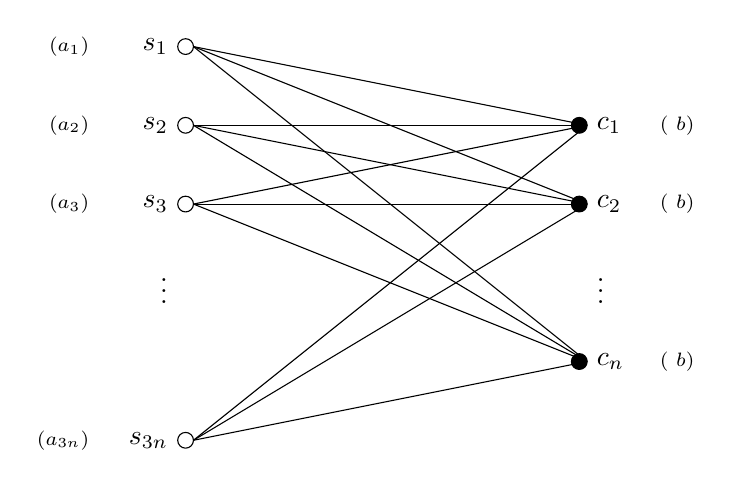
\begin{tikzpicture}
        \node[anchor=east] at (.4,8) {\(s_1\)};                                               \draw (.5,8) circle (.1);
        \node[anchor=east] at (.4,7) {\(s_2\)};                                               \draw (.5,7) circle (.1);   \draw[fill=black] (5.5,7) circle (.1);  \node[anchor=west] at (5.6,7) {\(c_1\)};
        \node[anchor=east] at (.4,6) {\(s_3\)};                                               \draw (.5,6) circle (.1);   \draw[fill=black] (5.5,6) circle (.1);  \node[anchor=west] at (5.6,6) {\(c_2\)};
        \node[anchor=east] at (.4,5) {\(\vdots\)};                                                                                                                                            \node[anchor=west] at (5.6,5) {\(\vdots\)};
                                                                                                                      \draw[fill=black] (5.5,4) circle (.1);  \node[anchor=west] at (5.6,4) {\(c_n\)};
        \node[anchor=east] at (.4,3) {\(s_{3n}\)};                                         \draw (.5,3) circle (.1);  

        \node[anchor=east] at (-.6,8) {\scriptsize (\(a_1\))};
        \node[anchor=east] at (-.6,7) {\scriptsize (\(a_2\))};        \node[anchor=west] at (6.4,7) {\scriptsize ( \(b\))};
        \node[anchor=east] at (-.6,6) {\scriptsize (\(a_3\))};        \node[anchor=west] at (6.4,6) {\scriptsize ( \(b\))};
                                                                                                      \node[anchor=west] at (6.4,4) {\scriptsize ( \(b\))};
        \node[anchor=east] at (-.6,3) {\scriptsize (\(a_{3n}\))};   

        \draw[-] (5.6,6) -- (.6,8);
        \draw[-] (5.6,6) -- (.6,7);
        \draw[-] (5.6,6) -- (.6,6);
        \draw[-] (5.6,6) -- (.6,3);
        
        \draw[-] (5.6,7) -- (.6,8);
        \draw[-] (5.6,7) -- (.6,7);
        \draw[-] (5.6,7) -- (.6,6);
        \draw[-] (5.6,7) -- (.6,3);
 
        \draw[-] (5.6,4) -- (.6,8);
        \draw[-] (5.6,4) -- (.6,7);
        \draw[-] (5.6,4) -- (.6,6);
        \draw[-] (5.6,4) -- (.6,3);
         
    \end{tikzpicture}
    \caption{Reduction of \textsc{3-partition} to d-CGPP.}\label{fig:bipartite}
\end{figure}

\edit{
    It is helpful to visualise this d-CGPP instance using a complete bipartite graph \(G\) (see \Cref{fig:bipartite}), in which the vertices on the left (``shelf-vertices'') represent the shelves and those on the right (``crop-vertices'') represent the crops. Each crop-vertex \(i\) has a supply of \(b\) units of flow and each shelf-vertex \(j\) has a capacity \(a_j\) representing the maximum amount of flow that can reach node \(j\).
    Sending one unit of flow on edge \(\{i,j\}\) models the assignment of one unit of crop \(i\) to shelf \(j\) and consumes one unit of its capacity \(a_j\).
    It is obvious that this d-CGPP instance is feasible if and only if we can send out all the supplies from the crop-vertices, in integer amounts, while respecting the shelf capacities and the configuration constraints, i.e., while ensuring that the flow reaching a shelf-vertex \(j\) originates from nodes \(i\) that model crops all requiring the same configuration.
    So, a solution of a d-CGPP instance with answer yes corresponds to an integer flow in \(G\).  
}    

\edit{
    We now claim that d-CGPP admits answer yes to the instance constructed above if and only if the given \textsc{3-partition} instance is a yes-instance.
    Indeed, suppose the d-CGPP instance constructed above admits answer yes and consider a corresponding flow in \(G\).
    \editt{\begin{enumerate}
        \item Because all crops require different configurations, each shelf-vertex must receive flow from at most one crop-vertex (otherwise the same shelf-vertex would require at least two different configurations).\label{it:hp1}
        \item Because \(b/4 < a_j < b/2, \; \forall j \in \{1,\ldots,3n\}\), each crop-vertex must send flow to at least 3 shelf-vertices (otherwise at least one capacity \(a_j\) would have to be greater or equal than \(b/2\)).\label{it:hp2}
        \item Because \(nb = \sum_{j=1}^{3n} a_j\), each shelf-vertex \(j\) must receive exactly \(a_j\) units of flow (otherwise the total flow received would be less than the flow sent).\label{it:hp3}
    \end{enumerate}
    Thus, using \ref{it:hp1}, \ref{it:hp2}, and \ref{it:hp3}, we can conclude that each crop-vertex must send its supply \(b\) to exactly three shelf-vertices.}
    In summary, an answer yes to d-CGPP implies that for each crop-vertex \(i=1, ..., n\), we can find a subset of exactly three shelf-vertices \(j\) whose capacities \(a_j\) sum to \(b\), and all these \(n\) subsets are disjoint.
    This yields the desired partition showing that the given \textsc{3-partition} instance is a yes-instance.
}

\edit{
    On the other hand, suppose that the given \textsc{3-partition} instance is a yes-instance implying the existence of a partition of \(A\) into \(n\) subsets \( A_1, \ldots, A_n\) that satisfy \(\sum_{a \in A_j} a = b, \; j = 1, \ldots, n\).
    Again, \(nb = \sum_{j=1}^{3n} a_j\)  and \(b/4 < a_j < b/2, \; \forall j \in \{1,\ldots,3n\}\) imply that each subset \(A_i\) contains three elements.
    We can then assign the \(b\) units of flow of each crop-vertex \(i\) to the three shelf-nodes with capacities in \(A_i\).
    Because the subsets \(A_i\) are disjoint, this yields an outflow of \(b\) units at each crop-vertex \(i\) and an inflow of \(a_j\) units at each shelf-vertex \(j\), all coming from the same node \(i\).
    Therefore, the d-CGPP instance has answer yes.
}

\edit{To conclude, we note that problem d-CGPP is in class \(\mathcal{NP}\), and that the described reduction is both polynomial and pseudo-polynomial.}

\section{Computational experiments}\label{sec:results}

This section describes the computational experiments on an extensive set of benchmark instances (see \Cref{ssec:instances} for a description)  to compare the performance of the different models (\Cref{ssec:performance}) and to investigate the structure of the solutions obtained with different objective functions (\Cref{ssec:comparison}).

\subsection{Benchmark instances and computational environment}\label{ssec:instances}

\begin{table}\centering%
    \begin{tabular}{@{}lccc@{}}
        \toprule
        {\bf cabinet} & {\bf \#shelves} & {\bf \#short shelves} & {\bf \#tall shelves} \\
        \midrule
        small  &  7 & 5 & 2 \\
        medium &  9 & 6 & 3 \\
        large  & 12 & 8 & 4 \\
        \bottomrule
    \end{tabular}
    \caption{%
        Features of the three types of cabinet considered.
        Column~\emph{cabinet} is the cabinet type.
        Column~\emph{\#shelves} report the total number of shelves in the cabinet, which is made up of the number of short and tall shelves, reported respectively in columns~\emph{\#short shelves} and \emph{\#tall shelves}.
        \label{tbl:cabinets}
    }
\end{table}

\begin{table}\centering%
    \begin{tabular}{@{}lccll@{}}
        \toprule
        {\bf crop} & {\bf total growth time} & {\bf \#growth phases} & {\bf shares config with} & {\bf shelf type} \\
        \midrule
        A & 64 & 3 & ---     & tall \\
        B & 15 & 2 & C, F    & short, tall \\
        C & 15 & 2 & B, F    & short, tall \\
        D & 44 & 5 & F       & short, tall \\
        E & 35 & 4 & ---     & short, tall \\
        F & 35 & 4 & B, C, D & short, tall \\
        \bottomrule        
    \end{tabular}
    \caption{%
        Real-life data about the crops that we used as a base for instance generation.
        Column~\emph{crop} is the crop identifier.
        Column~\emph{total growth time} gives the total time in days that the crop needs to be in the cabinet (quantity \(\gamma_c\)).
        Column~\emph{\#growth phases} is the number of different growth phases the crop goes through; each growth phase requires a different configuration.
        Column~\emph{shares config with} indicates which other crops
        have at least one required configuration in common with
        the considered crop (recall that crops which have common configurations can share the same shelf).
        Column~\emph{shelf type} states whether a crop can grow in any shelf or requires a tall one.
        \label{tbl:basedata}%
    }
\end{table}

We created a set of benchmark instances based on confidential real-life data, which we published online together with detailed results on an instance basis (see~\autocite{Repo}).
The base data contains information about crops and characteristics of commercial VF cabinets, and also includes historical demand data.
It assumes three types of cabinets containing different numbers of stacked shelves: small ones with seven shelves, medium ones with nine shelves, and large ones with twelve shelves.
The shelves can be of two types (short or tall), and \Cref{tbl:cabinets} shows how shelves are distributed in the cabinets.
Note that we do not report the capacity of the shelves because it varies with the configuration used (more concretely, it depends on the growth medium).
%In the rest of this section, we give details about the base data and the instance generation process.

We have data about six crops, which we denote using letters from \emph{A} to \emph{F}.
Crop \emph{A} requires tall shelves, while the other crops can grow on both short and tall shelves.
We handle this crop-to-shelf compatibility via parameters \(\delta_{ct}\) introduced in \Cref{sec:models}.
The crops we consider need between 15 and 64 days to grow, and go through two to five growth phases, with each phase corresponding to the need for a different configuration.
\Cref{tbl:basedata} reports the crop data in more detail: Column~\emph{total growth time} gives the total time in days that the crop needs to stay in the cabinet (parameter \(\gamma_c\)).
Column \emph{\#growth phases} is the number of different growth phases the crop goes through.
Column \emph{shares config with} indicates which other crops have at least one required configuration in common with the considered crop (recall that crops requiring the same configuration at the same time can share a shelf). Column \emph{shelf type} indicates whether a crop can grow in any shelf or requires a tall one.

\edit{The demand pattern is based on historical data and has a constant trend with weekly seasonality and some spikes on particular days (for example, holidays).}
Given the base data and this historical demand pattern, we generate new instances varying the number of crops considered and the time horizon length, and using a demand multiplier to simulate different demand situations:
\begin{itemize}
    \item We consider all possible combinations of crops, starting from instances with demand for only one crop, then considering the \(\binom{6}{2}\) possible ways of selecting two crops, etc.~up to instances with demand for all six crops.
    \item For each crop combination, we generate instances for the large, the medium, and the small cabinet.
    \item For each choice of crops and cabinet, we generate six instances by multiplying the base demand by a factor of \(1.0, 1.2, 1.4, 1.6, 1.8, 2.0\).
    \item For each choice of the three above parameters, we consider time horizons of 60, 80, and 100 days.
\end{itemize}
Given \(2^6 - 1 = 63\) possible ways to choose a crop combination (with at least one crop), 3 cabinets, 6 demand multiplier values, and 3 time horizon lengths, we have a total of 3402 instances.
Removing instances with a time horizon of 60 but containing crop \emph{A}, which needs 64 days to grow, leaves us with 2826 instances.

While all instances are feasible for model \emph{MinUD}, this is not true for the other models (\emph{MinM}, \emph{MinR} and \emph{MinS}).
Therefore, the first aim of our computational study was to determine which of the 2826 instances are feasible for the other three models (note that an instance is either feasible for all three or none of the models).
We coded the models using IBM ILOG Optimization Programming Language and ran them on a cluster equipped with Intel Xeon processors at 2.4GHz, reserving four cores and 4GB of RAM for each run.
We used the solver CPLEX 12.7 with a time limit of 1 hour and default settings.

\begin{table}\centering%
    \begin{tabular}{rrlrrrrr}
        \toprule
        \multicolumn{2}{c}{\bf \#crops} &%
        \multicolumn{2}{c}{\bf cabinet} &%
        \multicolumn{2}{c}{\bf demand mult} &%
        \multicolumn{2}{c}{\bf time horizon} \\
        value & \%feas & value & \%feas & value & \%feas & value & \%feas \\
        \cmidrule(lr){1-2}\cmidrule(lr){3-4}\cmidrule(lr){5-6}\cmidrule(lr){7-8}
        1 & 58.50 & small  & 41.61 & 1.0 & 66.03 &  60 & 82.80 \\
        2 & 61.39 & medium & 50.42 & 1.2 & 64.54 &  80 & 51.94 \\
        3 & 54.33 & large  & 61.04 & 1.4 & 57.96 & 100 & 34.48 \\
        4 & 41.90 &        &       & 1.6 & 46.50 &     &       \\
        5 & 26.07 &        &       & 1.8 & 43.74 &     &       \\
        6 & 19.44 &        &       & 2.0 & 27.39 &     &       \\
        \bottomrule
    \end{tabular}
    \caption{%
        Percentage of feasible instances when varying each of the four instance generation parameter.
        Column \emph{value} indicates the parameter value, while
        column \emph{\%feas} reports the number of feasible instances in percent.
        \label{tbl:feasible}%
    }
\end{table}

At the end of the runs, we determined that 1441 instances are feasible and 1382 are provably infeasible.
We were not able to establish the feasibility of the remaining 3 instances because CPLEX neither proved them infeasible nor produced a feasible solution within the time limit. 
\Cref{tbl:feasible} reports the relationship between the instance generation parameters  and the number of feasible instances.
Increasing the number of crops tends to decrease the number of feasible instances because crop demands are independent of each other: for example, instances with six crops have roughly twice the demand of instances with three crops.
Unsurprisingly, larger cabinets and lower demands lead to a higher number of feasible instances.
Finally, longer time horizons correspond to fewer feasible instances because it only takes one day with a surge in demand which the system cannot accommodate to render the whole instance infeasible; a longer time horizon corresponds to more opportunities for one such day.

\begin{sidewaystable}\centering\scriptsize%
    \resizebox{\textwidth}{!}{%
    \setlength{\tabcolsep}{3pt}
    \begin{tabular}{ll r rrrr rrrr rrrr rrrr}
        \toprule

        \multicolumn{2}{c}{\bf parameter} &
        {\bf instances} &
        \multicolumn{4}{c}{\bf MinM} &
        \multicolumn{4}{c}{\bf MinR} &
        \multicolumn{4}{c}{\bf MinS} &
        \multicolumn{4}{c}{\bf MinUD} \\

        \cmidrule(lr){1-2}
        \cmidrule(lr){3-3}
        \cmidrule(lr){4-7}
        \cmidrule(lr){8-11}
        \cmidrule(lr){12-15}
        \cmidrule(lr){16-19}

        {\bf name} & {\bf value} & &
        {\bf\%feas} & {\bf\%opt} & {\bf\%gap} & {\bf time} &
        {\bf\%feas} & {\bf\%opt} & {\bf\%gap} & {\bf time} &
        {\bf\%feas} & {\bf\%opt} & {\bf\%gap} & {\bf time} &
        {\bf\%feas} & {\bf\%opt} & {\bf\%gap} & {\bf time} \\
        

        \midrule

        \#crops &
        1 & 178 & 28.65 & 15.17 & 28.69 & 1899.30 & 61.80 & 56.74 & 6.80 & 11.99 & 100.00 & 100.00 & 0.00 & 5.89 & 100.00 & 100.00 & 0.00 & 0.71 \\
        & 2 & 442 & 37.56 & 2.71 & 79.40 & 3400.08 & 75.11 & 69.00 & 5.21 & 72.49 & 98.42 & 82.58 & 0.37 & 714.17 & 100.00 & 99.32 & 0.09 & 28.76 \\
        & 3 & 489 & 40.70 & 0.20 & 95.33 & 3600.00 & 74.85 & 71.17 & 2.30 & 172.69 & 98.98 & 45.40 & 2.68 & 2141.60 & 100.00 & 97.96 & 0.24 & 93.58 \\
        & 4 & 264 & 40.91 & 0.00 & 98.35 & 3600.00 & 75.00 & 72.35 & 0.94 & 209.26 & 97.73 & 12.50 & 7.06 & 3264.14 & 100.00 & 96.97 & 0.29 & 157.99 \\
        & 5 & 61 & 22.95 & 0.00 & 96.69 & 3600.00 & 85.25 & 81.97 & 1.13 & 417.50 & 98.36 & 1.64 & 10.76 & 3589.91 & 100.00 & 93.44 & 0.56 & 387.86 \\
        & 6 & 7 & 0.00 & 0.00 & --- & 3600.00 & 100.00 & 85.71 & 3.57 & 753.95 & 100.00 & 0.00 & 15.96 & 3600.00 & 100.00 & 85.71 & 1.19 & 558.28 \\


        \midrule

        cabinet&
        small & 391 & 41.43 & 4.35 & 75.60 & 3273.87 & 70.33 & 67.52 & 1.99 & 18.29 & 98.72 & 59.59 & 3.12 & 1591.38 & 100.00 & 99.49 & 0.08 & 32.86 \\
        & medium & 475 & 42.74 & 2.95 & 87.15 & 3393.94 & 72.42 & 68.00 & 5.60 & 53.88 & 98.53 & 53.89 & 3.00 & 1767.17 & 100.00 & 98.95 & 0.13 & 57.25 \\
        & large & 575 & 30.09 & 1.57 & 90.46 & 3497.95 & 77.57 & 72.00 & 2.49 & 299.21 & 98.78 & 53.91 & 2.52 & 1742.44 & 100.00 & 96.70 & 0.33 & 152.76 \\

        \midrule

        demand mult &
        1.0 & 311 & 50.80 & 3.54 & 86.58 & 3399.20 & 63.02 & 60.13 & 2.82 & 147.99 & 98.39 & 40.51 & 6.26 & 2250.36 & 100.00 & 98.07 & 0.19 & 96.42 \\
        & 1.2 & 304 & 46.71 & 3.29 & 86.16 & 3429.93 & 65.79 & 61.18 & 4.92 & 166.05 & 97.37 & 48.68 & 3.52 & 1916.93 & 100.00 & 97.37 & 0.28 & 120.99 \\
        & 1.4 & 273 & 38.10 & 1.83 & 88.00 & 3467.99 & 75.09 & 71.43 & 3.76 & 94.55 & 98.90 & 56.04 & 2.12 & 1729.95 & 100.00 & 98.53 & 0.15 & 84.04 \\
        & 1.6 & 218 & 27.52 & 1.83 & 83.51 & 3393.07 & 82.11 & 78.44 & 2.61 & 140.36 & 100.00 & 62.39 & 1.41 & 1467.36 & 100.00 & 99.54 & 0.07 & 43.78 \\
        & 1.8 & 206 & 23.30 & 3.88 & 75.83 & 3106.17 & 81.07 & 74.27 & 3.19 & 157.94 & 99.51 & 65.53 & 0.80 & 1360.96 & 100.00 & 96.60 & 0.37 & 134.90 \\
        & 2.0 & 129 & 20.16 & 1.55 & 72.06 & 3346.49 & 91.47 & 84.50 & 2.37 & 202.66 & 98.45 & 78.29 & 0.29 & 858.51 & 100.00 & 100.00 & 0.00 & 6.46 \\

        \midrule

        time horizon &
        60 & 461 & 42.52 & 2.60 & 86.56 & 3432.42 & 79.39 & 78.09 & 1.14 & 43.57 & 99.78 & 74.40 & 1.45 & 1051.89 & 100.00 & 98.92 & 0.13 & 56.38 \\
        &  80 & 589 & 39.05 & 3.57 & 84.38 & 3340.80 & 70.63 & 65.87 & 4.14 & 119.48 & 98.30 & 53.99 & 2.78 & 1771.87 & 100.00 & 97.45 & 0.26 & 108.92 \\
        & 100 & 391 & 28.64 & 1.79 & 82.28 & 3422.71 & 72.38 & 64.71 & 5.11 & 322.84 & 97.95 & 35.29 & 4.60 & 2405.31 & 100.00 & 98.47 & 0.17 & 96.49 \\

        \midrule

        \multicolumn{2}{l}{Overall} & 1441 & 37.34 & 2.78 & 84.74 & 3391.23 & 73.91 & 69.47 & 3.37 & 147.43 & 98.68 & 55.45 & 2.84 & 1709.58 & 100.00 & 98.20 & 0.19 & 88.74 \\

        \bottomrule
    \end{tabular}}
    \caption{%
        Performance comparison of the four models for varying instance parameters.
        Column \emph{instances} reports how many instances, out of those identified as feasible in \Cref{ssec:instances}, correspond to the setting specified under \emph{parameter}.
        Column \emph{\%feas} indicates the number of instances (in percent) for which the model produced a feasible solution.
        Column \emph{\%opt} lists the number of instances solved to optimality  in percent.
        Column \emph{\%gap} reports the average optimality gap in percent, and column \emph{time} is the average solution time in seconds.
        The last two columns are computed based on the instances with a feasible solution found within the time limit.%
    }\label{tbl:model_performance}
\end{sidewaystable}

\subsection{Performance of the models}\label{ssec:performance}

In this section, we investigate the performance of each of the four models and analyse the effect of the instance parameters (number of crops, cabinet type, demand multiplier, time horizon) on this performance.
\Cref{tbl:model_performance} reports the results of the models based on the set of 1441 instances that we proved to be feasible for all models.
The five parts of the table show the results in aggregated form (grouped according to different settings of the instance parameters and as overall aggregate).
For each value of instance parameter, column \emph{instances} reports the number of instances aggregated in the row.
For each model, column \emph{\%feas} reports the percentage of instances for which the respective model found a feasible solution within the 1-hour time limit. Column \emph{\%opt} reports the percentage of instances solved to optimality, column \emph{\%gap} the average optimality gap in percent, and column \emph{time} the average runtime of CPLEX in seconds. 
Columns \emph{\%gap} and \emph{time} are computed based on the instances with a feasible solution found by the respective model within the time limit.

Of the stricter models, i.e., those models in which demand has to be met, \emph{MinM} shows the worst performance.
It provides the fewest instances with a feasible solution (in fact, for the large majority of instances, CPLEX cannot produce a feasible solution within the time limit), the largest optimality gaps, and the highest runtimes.
This is due to the fact that, in this model, we cannot aggregate shelves into shelf types, leading to considerably more variables and constraints.
A higher number of crops (beyond four), larger cabinets, higher demands, and longer time horizons have a clear negative effect on the ability of the model to find feasible solutions.
The effect of the instance parameters on solution quality is rather small and not always monotonic, which can be explained by the generally weak performance of the model on nearly all instances. 

With regards to finding feasible solutions, we observe a clear improvement for model \emph{MinR} and again for \emph{MinS}.
However, even for \emph{MinS}, instances exist for which no feasible solution can be determined within the time limit.
This highlights the necessity of alternative solution approaches to provide the planner with at least one feasible solution to implement. 
While the instance parameters have only a very slight impact on the feasibility of solutions for \emph{MinS}, for \emph{MinR}, a higher number of crops, larger cabinets, and higher demands clearly increase feasibility (the effect of longer time horizons is unclear). A possible explanation is that larger cabinets correspond to a larger solution space, which can be harder to explore but can make it easier to find a feasible solution.

Concerning solution quality, \emph{MinR} finds more optimal solutions within clearly shorter runtimes than \emph{MinS} while average gaps are slightly larger.
The performance difference between these two models strongly depends on instance parameters.
A higher number of crops clearly improves solution quality for the former model while strongly decreasing it for the latter.
This is due to the poor behaviour of variables \(y\) in the linear relaxation of all models, which is caused by \editt{capacity and linking} constraints~\eqref{eq:capacity}.
\editt{To better illustrate the impact of these constraints, in \Cref{app:capacity} we present an example of how constraints~\eqref{eq:capacity} lead to a linear relaxation solution with a 100\% gap to optimal integer solution.}
The poor behaviour of \eqref{eq:capacity} is exacerbated when shelves operate near full capacity and few shelves can be empty, e.g., when considering a large number of crops or longer time horizons.
In this case, many \(y\) variables will be non-zero and will take fractional values close to, but strictly less than one in the linear relaxation, thus requiring more branching.
In model \emph{MinS}, the objective function indirectly penalises variables \(y\) through variables \(v\), which therefore tend to assume fractional values more often, leading to worse performance.
Larger cabinets have a slightly positive effect on \emph{MinR} and a slightly negative effect on \emph{MinS}; higher demands increase solution quality for both models.

Contrary to these observations, the less strict model \emph{MinUD} always produces feasible solutions with ease (for example, a solution not growing anything is feasible).
It also shows the highest percentage of instances solved to optimality and the lowest average gaps, confirming that solving the model with a commercial solver is a valid approach to the CGPP when minimising unmet demand.
A higher number of crops and larger cabinets decrease solution quality while the effect of higher demands and longer time horizons is small and unclear.

\editt{If for the other objectives, {\em MinM}, {\em MinR} or {\em MinS}, instances are infeasible or it is not possible to find a feasible solution in reasonable runtime, the following simple strategy can be used to provide decision support. We first solve the {\em MinUD} model to obtain a subset of crops which are guaranteed to satisfy the capacity constraints of the VF system. Then, the original objective function can be used on an instance only containing the crops selected by {\em MinUD}. If it is still hard to find a feasible solution of the problem instance, the solution produced by model {\em MinUD} can be used as a last resort.}


\begin{figure}[htbp]\centering
    \begin{subfigure}[t]{.5\textwidth}
        \includegraphics[width=\textwidth]{reconfigurations}
        \caption{Number of reconfigurations per shelf.}\label{fig:reconfigurations}
    \end{subfigure}%
    \begin{subfigure}[t]{.5\textwidth}
        \includegraphics[width=\textwidth]{movements}
        \caption{Number of crop movements per unit of crop grown in the system.}\label{fig:movements}
    \end{subfigure}\\[2em]
    \begin{subfigure}[t]{.5\textwidth}
        \includegraphics[width=\textwidth]{used-shelves}
        \caption{Share of shelves used.}\label{fig:used-shelves}
    \end{subfigure}
    \caption{Each box spans the second and the third quartiles, with whiskers extending to the rest of the distribution (excluding outliers).
    The horizontal black line inside each box depicts the median.
    Each dot represents one instance.}
\end{figure}

\subsection{Effect of different objective functions}\label{ssec:comparison}

In this section, we investigate the impact of optimising with regards to a certain objective function on the structure of the resulting solutions.
More precisely, we want to see to what extent the characteristics stipulated by the other objective functions can already be witnessed in the solutions, i.e., whether the studied objectives are synergic or contradictory.
To this end, we recorded the number of crop movements, reconfigurations, and used shelves in the solutions of all models.
\Cref{fig:movements,fig:reconfigurations,fig:used-shelves} report the information about, respectively, the number of reconfigurations per shelf, the number of movements per unit of crop, and the fraction of shelves used in the solutions found by the different models.

In all the figures, we note that only the model minimising the given objective achieves satisfactory results.
In \Cref{fig:reconfigurations}, the models which do not minimise the number of reconfigurations give solutions with a median of up to twenty reconfigurations per shelf and model; \emph{MinS} even has outliers with up to 60 reconfigurations per shelf.
Intuitively, indeed, if a planner wants to minimise the number of used shelves, he has to juggle as many configurations as possible in the few active shelves, which makes these two objectives contradictory.
We can observe the same effect in \Cref{fig:movements}: when minimising the number of shelves the planner has to frequently move around crops.
Finally, \Cref{fig:used-shelves} shows that when shelf minimisation is not explicitly demanded by the objective function, the models try to use as many shelves as possible: all models except \emph{MinS} have median shelf usage of 100\%.


\edit{
    To attempt to reconcile the objectives \emph{MinR} and \emph{MinS}, we investigate the effect of using a hierarchical objective which first minimises the number of reconfigurations and then the number of shelves used.
    The hierarchical objective reduces average shelf usage over all instances from 93.2\% (without hierarchical objective) to 92.4\%.
    This shows that the objectives are inherently conflicting, which makes a multi-objective approach compelling for practitioners, who want to achieve different desirable objectives simultaneously.
    The planner can clearly not rely on the assumption that optimising with regards to one objective will produce solutions of acceptable quality with respect to any other objective.
}

\section{Conclusions}\label{sec:conclusions}

In this paper, we present four mathematical models for planning the growth of crops in a vertical farming system, which are strengthened using variable fixing and valid inequalities.
The models mainly differ in their objective to minimise, respectively, movements, reconfigurations, shelf usage, or unmet demand.
Numerical experiments on a large set of benchmark instances based on real-world data show that the performance of the models when solved with a standard solver is diverse and strongly dependent on instance data.
\edit{In particular, when minimising the number of crop movements, we cannot solve to optimality more than 97\% of the instances, and the average gaps are above 84\%.
By contrast, average gaps are below 4\% for the other objectives.
This suggests that developing ad-hoc algorithms to minimise the number of movements is an interesting area for future research.}

We also find that none of the objectives steers the solutions to be acceptable with regards to any of the other objectives, which makes multi-objective optimisation techniques another fruitful avenue for future investigations.
\edit{In this work, we assume that, because the crops are highly perishable, their growth should complete on the same day in which there is demand for them.
This is particularly true for crops currently popular for VF systems, such as basil, chives, or leafy greens.
As VF technology improves, however, the range of crops which one can grow in a controlled-condition cabinet will increase.
In this case, a promising research direction is to allow some crop units to be harvested before their due date thereby introducing flexibility in the time when their growth is started. This clearly adds a scheduling component to our model.
Such a research direction would benefit the area of machine scheduling in general, because there are currently no other models allowing such a great flexibility in reconfiguring machines and moving tasks between machines.}

\section*{Acknowledgements}

The authors are extremely grateful to Julia Bennell, Toni Martinez, and Chris Potts for sharing with us the slides of their presentation at the MIC'17 conference~\autocite{potts2017vf}.

\printbibliography

\appendix

\section{Complete models}\label{app:models}

In this section we provide complete models for the four formulations presented in \Cref{sec:models}.

\subsection{Minimise the number of movements}

\begin{align}
    \min &
    \sum_{c \in C} \sum_{g = 1}^{\gamma_c} \sum_{\substack{s1, s2 \in S_c \\ s_1 \neq s_2}} \sum_{d \in D}
    \xvar{s_1}{d}{s_2}{c}{g} \\
    \text{s.t.} &
    \sum_{s \in S_c} \xvar{s}{d-1}{\tau}{c}{\gamma_c} = p_{cd} & \quad &
    \forall c \in C, \forall d \in D \cup \{\bar{d}\} \\
    &
    \sum_{s_2 \in S'} \sum_{\substack{c \in C \\ \delta_{c s_1} = 1 \\ \delta_{c s_2} = 1}} \sum_{\substack{g \in \{1,\ldots,\gamma_c\} \\ k_{c,g} = k}} \xvar{s_1}{d}{s_2}{c}{g} \leq
    q_{s_1 k} \cdot \yvar{s_1}{d}{k} & \quad &
    \forall s_1 \in S, \forall d \in D, \forall k \in K \\
    &
    \sum_{s \in S_c} \xvar{\sigma}{d - \gamma_c - 1}{s}{c}{0} = p_{cd} & \quad &
    \forall c \in C, \forall d \in \{ \gamma_c + 1, \ldots, \bar{d} \} \\
    &
    \sum_{s_2 \in T'_c} \xvar{s_2}{d-1}{s_1}{c}{g} =
    \sum_{s_2 \in T'_c} \xvar{s_1}{d}{s_2}{c}{g+1} & \quad &
    \forall c \in C, \forall g \in \{0,\ldots,\gamma_c\}, \forall s_1 \in S_c, \forall d \in D \\
    &
    \sum_{k \in K} \yvar{s}{d}{k} \leq 1 & \quad &
    \forall s \in S, \forall d \in D \\
    &
    \xvar{s_1}{d}{s_2}{c}{g} \in \mathbb{N} & \quad &
    \forall c \in C, \;
    \forall s_1, s_2 \in S'_c, \;
    \forall d \in D', \;
    \forall g \in \{0, \ldots, \gamma_c\} \\
    &
    \yvar{s}{d}{k} \in \{0,1\} & \quad &
    \forall s \in S'_c, \;
    \forall d \in D', \;
    \forall k \in K
\end{align}

\subsection{Minimise the number of reconfigurations}

\begin{align}
    \min &
    \sum_{t \in T} \sum_{d = 1}^{\bar{d} - 2} \sum_{k \in K} \wvar{t}{d}{k} \\
    \text{s.t.} &
    \sum_{t \in T_c} \xvar{t}{d-1}{\tau}{c}{\gamma_c} = p_{cd} & \quad &
    \forall c \in C, \forall d \in D \cup \{\bar{d}\} \\
    &
    \sum_{t_2 \in T'} \sum_{\substack{c \in C \\ \delta_{c t_1} = 1 \\ \delta_{c t_2} = 1}} \sum_{\substack{g \in \{1,\ldots,\gamma_c\} \\ k_{c,g} = k}} \xvar{t_1}{d}{t_2}{c}{g} \leq
    q_{t_1 k} \cdot \yvar{t_1}{d}{k} & \quad &
    \forall t_1 \in T, \forall d \in D, \forall k \in K \\
    &
    \sum_{t \in T_c} \xvar{\sigma}{d - \gamma_c - 1}{t}{c}{0} = p_{cd} & \quad &
    \forall c \in C, \forall d \in \{ \gamma_c + 1, \ldots, \bar{d} \} \\
    &
    \sum_{t_2 \in T'_c} \xvar{t_2}{d-1}{t_1}{c}{g} =
    \sum_{t_2 \in T'_c} \xvar{t_1}{d}{t_2}{c}{g+1} & \quad &
    \forall c \in C, \forall g \in \{0,\ldots,\gamma_c\}, \forall t_1 \in T_c, \forall d \in D \\
    &
    \sum_{k \in K} \yvar{t}{d}{k} \leq n_t & \quad &
    \forall t \in T, \forall d \in D \\
    &
    \wvar{t}{d}{k} \geq \yvar{t}{d}{k} - \yvar{t}{d+1}{k} & \quad &
    \forall t \in T, \; \forall d \in \{ 1, \ldots, \bar{d} - 2 \}, \; \forall k \in K \\
    &
    \wvar{t}{d}{k} \geq \yvar{t}{d+1}{k} - \yvar{t}{d}{k} & \quad &
    \forall t \in T, \; \forall d \in \{ 1, \ldots, \bar{d} - 2 \}, \; \forall k \in K \\
    &
    \xvar{t_1}{d}{t_2}{c}{g} \in \mathbb{N} & \quad &
    \forall c \in C, \;
    \forall t_1, t_2 \in T'_c, \;
    \forall d \in D', \;
    \forall g \in \{0, \ldots, \gamma_c\} \\
    &
    \yvar{t}{d}{k} \in \mathbb{N} & \quad &
    \forall t \in T'_c, \;
    \forall d \in D', \;
    \forall k \in K \\
    & \wvar{t}{d}{k} \in \mathbb{N} & \quad &
    \forall t \in T, \;
    \forall d \in \{1, \ldots, \bar{d}-2\}, \;
    \forall k \in K
\end{align}

\subsection{Minimise unmet demand}

\begin{align}
    \min &
    \sum_{c \in C} \sum_{d = 1}^{\bar{d}} \omega_{cd} \uvar{c}{d} \\
    \text{s.t.} &
    \sum_{t \in T_c} \xvar{t}{d-1}{\tau}{c}{\gamma_c} + \uvar{c}{d} = p_{cd} & \quad &
    \forall c \in C,  \forall d \in D \cup \{\bar{d}\} \\
    &
    \sum_{t_2 \in T'} \sum_{\substack{c \in C \\ \delta_{c t_1} = 1 \\ \delta_{c t_2} = 1}} \sum_{\substack{g \in \{1,\ldots,\gamma_c\} \\ k_{c,g} = k}} \xvar{t_1}{d}{t_2}{c}{g} \leq
    q_{t_1 k} \cdot \yvar{t_1}{d}{k} & \quad &
    \forall t_1 \in T, \forall d \in D, \forall k \in K \\
    &
    \sum_{t \in T_c} \xvar{\sigma}{d - \gamma_c - 1}{t}{c}{0} + \uvar{c}{d} = p_{cd} & \quad &
    \forall c \in C, \forall d \in \{ \gamma_c + 1, \ldots, \bar{d} \} \\
    &
    \sum_{t_2 \in T'_c} \xvar{t_2}{d-1}{t_1}{c}{g} =
    \sum_{t_2 \in T'_c} \xvar{t_1}{d}{t_2}{c}{g+1} & \quad &
    \forall c \in C, \forall g \in \{0,\ldots,\gamma_c\}, \forall t_1 \in T_c, \forall d \in D \\
    &
    \sum_{k \in K} \yvar{t}{d}{k} \leq n_t & \quad &
    \forall t \in T, \forall d \in D \\
    &
    \xvar{t_1}{d}{t_2}{c}{g} \in \mathbb{N} & \quad &
    \forall c \in C, \;
    \forall t_1, t_2 \in T'_c, \;
    \forall d \in D', \;
    \forall g \in \{0, \ldots, \gamma_c\} \\
    &
    \yvar{t}{d}{k} \in \mathbb{N} & \quad &
    \forall t \in T'_c, \;
    \forall d \in D', \;
    \forall k \in K \\
    &
    \uvar{c}{d} \in \mathbb{N} & \quad &
    \forall c \in C, \;
    \forall d \in D \cup \{ \bar{d} \}
\end{align}

\subsection{Minimise the number of shelves used}

\begin{align}
    \min &
    \sum_{t \in T} v_t \\
    \text{s.t.} &
    \sum_{t \in T_c} \xvar{t}{d-1}{\tau}{c}{\gamma_c} = p_{cd} & \quad &
    \forall c \in C, \forall d \in D \cup \{\bar{d}\} \\
    &
    \sum_{t_2 \in T'} \sum_{\substack{c \in C \\ \delta_{c t_1} = 1 \\ \delta_{c t_2} = 1}} \sum_{\substack{g \in \{1,\ldots,\gamma_c\} \\ k_{c,g} = k}} \xvar{t_1}{d}{t_2}{c}{g} \leq
    q_{t_1 k} \cdot \yvar{t_1}{d}{k} & \quad &
    \forall t_1 \in T, \forall d \in D, \forall k \in K \\
    &
    \sum_{t \in T_c} \xvar{\sigma}{d - \gamma_c - 1}{t}{c}{0} = p_{cd} & \quad &
    \forall c \in C, \forall d \in \{ \gamma_c + 1, \ldots, \bar{d} \} \\
    &
    \sum_{t_2 \in T'_c} \xvar{t_2}{d-1}{t_1}{c}{g} =
    \sum_{t_2 \in T'_c} \xvar{t_1}{d}{t_2}{c}{g+1} & \quad &
    \forall c \in C, \forall g \in \{0,\ldots,\gamma_c\}, \forall t_1 \in T_c, \forall d \in D \\
    &
    \sum_{k \in K} \yvar{t}{d}{k} \leq n_t & \quad &
    \forall t \in T, \forall d \in D \\
    &
    v_t \geq \sum_{k \in K \setminus \{ k_0 \}} \yvar{t}{d}{k} & \quad & \forall t \in T, \forall d \in D \\
    &
    \xvar{t_1}{d}{t_2}{c}{g} \in \mathbb{N} & \quad &
    \forall c \in C, \;
    \forall t_1, t_2 \in T'_c, \;
    \forall d \in D', \;
    \forall g \in \{0, \ldots, \gamma_c\} \\
    &
    \yvar{t}{d}{k} \in \mathbb{N} & \quad &
    \forall t \in T'_c, \;
    \forall d \in D', \;
    \forall k \in K \\
    &
    v_t \in \mathbb{N} & \quad &
    \forall t \in T
\end{align}

\section{Example of solution of the continuous relaxation of model {\bf MinM}}\label{app:capacity}

A disadvantage of the proposed formulations is their weak linear relaxation, mainly due to the presence of constraints ~\eqref{eq:capacity}.
These inequalities serve both as capacity constraints and as linking constraints for the \(x\)- and \(y\)-variables, but they provide a weak linking between these variables once the integrality requirements are removed.

\begin{figure}[ptbh]\centering
    \begin{subfigure}[b]{0.475\textwidth}\centering
        \resizebox{.75\textwidth}{!}{\begin{tikzpicture}
    \foreach \x in {0,...,3}
        \node at (2 * \x, 8) {\(d=\x\)};

    \node at (-2, 6) {\(\sigma\)};

    \foreach \y in {1,...,2} {
        \pgfmathtruncatemacro{\ylabel}{3-\y}
        \node at (-2, 2 * \y) {shelf \ylabel};
    };

    \node at (-2, 0) {\(\tau\)};

    \foreach \x in {0,...,3}
        \foreach \y in {0,...,3}
            \draw[black,fill=black] (2 * \x, 2 * \y) circle (.5ex) node (p\x\y) {};
            
    \path[->,dashed]
        (p03) edge (p12)
        (p12) edge (p22)
        (p22) edge[transform canvas={yshift=.05cm,xshift=.05cm}] (p30);
        
    \path[->,dotted]
        (p03) edge (p11)
        (p11) edge (p22)
        (p22) edge[transform canvas={yshift=-.05cm,xshift=-.05cm}] (p30);
        
    \path[->]
        (p13) edge (p21)
        (p21) edge (p30);
        
    \node[below left=-.1cm and -.3cm of p12] {\small \(k_1\)};
    \node[above right=-.1cm and -.3cm of p22] {\small \(k_2\)};
    \node[below left=-.1cm and -.3cm of p11] {\small \(k_3\)};
    \node[below left=-.1cm and -.3cm of p21] {\small \(k_4\)};
\end{tikzpicture}}
        \caption{Optimal solution for model {\bf MinM}.}\label{fig:exbigm1}
    \end{subfigure}%
    \hfill%
     \begin{subfigure}[b]{0.475\textwidth}\centering
        \resizebox{.75\textwidth}{!}{\input{example-bigM2}}
        \caption{Optimal solution of the continuous relaxation of model {\bf MinM}.}\label{fig:exbigm2}
    \end{subfigure}%
    \caption{Example instance in which the continuous relaxation of model {\bf MinM} would show a gap of 100\%.}\label{fig:exbigm}
\end{figure}

To illustrate this point consider model {\bf MinM} and an instance with two identical shelves of capacity \(2\) and three crops:
\begin{itemize}
    \item crop \(c_1\) is planted on day 0 and grows for two days, in configuration \(k_1\) on the first day and in \(k_2\) on the second;
    \item crop \(c_2\) is also planted on day 0 and grows for two days, in configuration \(k_3\) on the first day and in \(k_2\) on the second;
    \item crop \(c_3\) is planted on day 1 and grows for one day in configuration \(k_4\).
\end{itemize}
Each crop has demand 1 only on the third day.
\Cref{fig:exbigm1} shows an optimal solution to this instance. In the figure, the movements of crop \(c_1\) are visualised as dashed arrows, those of crop \(c_2\) as dotted arrows and those of crop \(c_3\) as solid arrows. Note that the objective value of this solution is 1, because crop \(c_2\) moves from shelf \(s_2\) to \(s_1\) in day 2.
The value of the non-zero variables in this optimal solution is: \(\xvar{\sigma}{0}{s_1}{c_1}{0} = \xvar{s_1}{1}{s_1}{c_1}{1} = \xvar{s_1}{2}{\tau}{c_1}{2} = \xvar{\sigma}{0}{s_2}{c_2}{0} = \xvar{s_2}{1}{s_1}{c_2}{1} = \xvar{s_1}{2}{\tau}{c_2}{2} = \xvar{\sigma}{1}{s_2}{c_3}{0} = \xvar{s_2}{2}{\tau}{c_3}{1} = 1\) and \(\yvar{s_1}{1}{k_1} = \yvar{s_1}{2}{k_2} = \yvar{s_2}{1}{k_3} = \yvar{s_2}{2}{k_4} = 1\).

On the other hand, if we consider the continuous relaxation, we can obtain a solution with an objective value equal to zero thus yielding an integrality gap of \(100\%\).
Such a solution is shown in \Cref{fig:exbigm2}.
Here, shelf \(s_1\) can be assigned half configuration \(k_1\) and half configuration \(k_3\) on day \(1\) because variables \(\yvar{s_1}{1}{k_1}\) and \(\yvar{s_1}{1}{k_3}\) can both be given a value 0.5.
Since the shelf capacity is \(2\) it can accommodate both crops \(c_1\) and \(c_2\) simultaneously and with these fractional values for variables \(\yvar{s_1}{1}{k_1}\) and \(\yvar{s_1}{1}{k_3}\) constraints \eqref{eq:capacity} are indeed satisfied.

Overall, the value of the non-zero variables in the optimal solution to the linear relaxation is: \(\xvar{\sigma}{0}{s_1}{c_1}{0} = \xvar{s_1}{1}{s_1}{c_1}{1} = \xvar{s_1}{2}{\tau}{c_1}{2} = \xvar{\sigma}{0}{s_1}{c_2}{0} = \xvar{s_1}{1}{s_1}{c_2}{1} = \xvar{s_1}{2}{\tau}{c_2}{2} = \xvar{\sigma}{1}{s_2}{c_3}{0} = \xvar{s_2}{2}{\tau}{c_3}{1} = 1\), \(\yvar{s_1}{1}{k_1} = \yvar{s_1}{1}{k_3} = 0.5\) and \(\yvar{s_1}{2}{k_2} = \yvar{s_2}{2}{k_4} = 1\). As noted above, this solution does not violate constraints \eqref{eq:capacity}, nor the other linear constraints of the model.

\end{document}